\documentclass[11pt,singleside]{myfithesis2}
\usepackage[hyphens]{url}
\usepackage[english]{babel}  %  package  for  multilingual  support
\usepackage[utf8]{inputenc}  %  UTF-8  encoding
\usepackage[IL2]{fontenc}
\usepackage[plainpages=false,pdfpagelabels,unicode]{hyperref}
\usepackage{fancyvrb}
\usepackage{graphicx}
\usepackage{listings}
\usepackage{color}
\usepackage{textcomp}
\usepackage[small]{caption}
\usepackage{float}
\usepackage{verbatim}
\usepackage{pdfpages}
 
\definecolor{listinggray}{gray}{0.9}
\definecolor{lbcolor}{rgb}{0.9,0.9,0.9}
\definecolor{darkgray}{gray}{0.3}
\definecolor{palegray}{gray}{0.85}

\hyphenation{YSoft SafeQ Sikuli Soft}

\lstset{
	numbers=left,
	backgroundcolor=\color{lbcolor},
	tabsize=4,
	rulecolor=,
	language=java,
       basicstyle=\footnotesize,
       %basicstyle=\ttfamily,
       upquote=true,
       aboveskip={\baselineskip},
       %belowskip={\baselineskip},
       columns=fixed,
       showstringspaces=false,
       extendedchars=true,
       breaklines=true,
       prebreak = \raisebox{0ex}[0ex][0ex]{\ensuremath{\hookleftarrow}},
       frame=tb,
       showtabs=false,
       showspaces=false,
       showstringspaces=false,
       identifierstyle=\ttfamily,
       keywordstyle=\color[rgb]{0,0,1},
       commentstyle=\color[rgb]{0.133,0.545,0.133},
       stringstyle=\color[rgb]{0.627,0.126,0.941},
	emph=, emphstyle=\color{black},
	captionpos=b,
}



\newcommand{\pict}[4]{
	\begin{figure}[h!]
  		\vspace{-7px}
  		\centerline{\fcolorbox{darkgray}{palegray}{\includegraphics[#3]{#2}}}
  		\caption{#1}
  		\label{#4}
	\end{figure}
}

\makeatletter
\renewcommand\paragraph{
   \vspace{-10pt}
   \@startsection{paragraph}{4}{0mm}
      {\baselineskip}
      {- 5pt}
      {\normalfont\normalsize\bfseries}
}
\makeatother
\renewcommand\lstlistingname{Source code}
\renewcommand\lstlistlistingname{List of source codes}

\hypersetup{
    colorlinks,
    citecolor=black,
    filecolor=black,
    linkcolor=black,
    urlcolor=black
}

\clubpenalty=10000
\widowpenalty=10000
\thesistitle{Making Internal Communication in~a~Software Company More~Efficient}  %  thesis  title
\thesissubtitle{Diploma thesis}
\thesisstudent{Martin Bryndza}        %  name  of  the  author
\thesiswoman{false} %  defines  author’s  gender
\thesisfaculty{fi}
\thesisyear{2015}
\thesisadvisor{Mgr. Peter Neugebauer, MBA}  %  fill  in  advisor’s  name
\thesislang{en} %  thesis  is  in  English
\begin{document}
\FrontMatter
\ThesisTitlePage
\begin{ThesisDeclaration}
\DeclarationText
\AdvisorName
\end{ThesisDeclaration}
\begin{ThesisThanks}
I would like to thank to my supervisor Mgr. Petr Neugebauer, MBA for his valuable advices and guidance. Great thanks go to the Y Soft Corporation for giving me the opportunity to perform the unnecessary research. Many thanks also go to my colleagues from the ETNA team, who contributed to this thesis with their cooperation and willingness to try new things. These are the people who agreed to do some extra work without hesitation. I would like to send many thanks also to my colleagues from the QA team for their support in the last months of me working on this thesis. With their help I was able to have enough time for the thesis while also getting all the planned work done for each sprint. Last but not least, I would like to thank to my dear Marie for her love and patience she had with me working overnight and also to my parents for their support throughout my studies. 
\end{ThesisThanks}
\begin{ThesisAbstract}
The goal of this thesis is to streamline communication between team members and to prevent loss of productivity due to frequent interruptions in a mid-size software company, where employers are dealing with adaptation of agile approaches. The thesis should analyze internal processes as well as requirements and expectations of different stakeholders regarding productivity, especially communication gaps. Based on these identified issues, the implementation part of the work will cover design and implementation of a tool, which will enforce the team members to follow the proposed process(es). This thesis is realized in cooperation with Y Soft Corporation, a.s.
\end{ThesisAbstract}
\begin{ThesisKeyWords}
Agile, AnyOffice, Communication, Company, Interruption, Team, Teamwork.
\end{ThesisKeyWords}
\MainMatter
\tableofcontents %  prints  table  of  contents
%\listoffigures % prints list of pictures
%\lstlistoflistings % prints list of blocks of code
%\listoftables % prints list of tables

\chapter{Introduction}

Agile frameworks overview, benefits of agile approaches => communication (From ISTQB syllabus)

scrum diagram

http://www.agilemodeling.com/essays/communication.htm
Communication is the act of transmitting information between individuals. The need to communicate effectively pervades software development, operations, and support. Developers and end users must communicate with one another. Developers and operations staff must communicate. Developers and management must communicate. And so on.




\chapter{Effective Work}

This chapter will give you an insight on what an interruption means to a programmer. The reasoning will be supported with a few researches bringing interesting results of the real cost of interruptions. In the second part, you can find a short summary of The Pomodoro Technique, which can help reducing interruptions and boosting up productivity. The section also contains a list of objectives, that are necessary, in order to implement the technique into your work customs.

	\section{The Cost of Interruptions}
Interruptions are a big source of inefficiency for everybody. For programmers, it is even more difficult to start where they finished prior to the interruption.

		\subsection{What It Means To Interrupt a Programmer}
In a company, there are positions, for which interruptions are just a normal part of the day. Sometimes, interruptions are what their work is mostly based on. A nice representation of this group are managers, who constantly change focus throughout the day. Their time is usually spit up in one hour intervals, each of them containing a single task. Likewise, if we take people from marketing. An interruption for them means a time spent dealing with the interruption and a few seconds more to find out where they had finished. For programmers, it is much more different.

A comic made by Jason Heeris, which you can find in the Appendix on page \pageref{app:programmer},  is probably the best way to give you an idea about what it means for a programmer to be interrupted. Imagine a programmer in a middle of a debugging task. He has finally come to a sufficient level of understanding of the tricky condition in the code, has done the right amount of cycles to get the correct value in a variable, which purpose is a little mystery to him, and is very probably just about to find out, what causes the exception, that the important customer sees in logs from time to time under unknown conditions. All of a sudden, a colleague comes by to ask about that other task the programmer had been working on and is currently under test. The distraction causes him to accidentally step over the expression instead of stepping into it. So, he asks the colleague to repeat the question, as he was only partly listening. After helping the colleague, he looks down at his paper wondering, what `'18rts97'' means, and restarts the debugging process.

Erik Dietrich in an article on his blog \cite{costOfInterruptions} provides a simple way of showing, what it means for a developer to be interrupted:\newline
Write down a series of 3 to 4 digit numbers in a sequence. Now, tell the person to add those numbers as fast as possible without writing anything down. After some time, ask the person questions about how it is going, what number he/she is currently adding, whether it is 198 or 674 and get him/her to respond. Ask him to help you with adding some other three numbers real quick. Moreover, you can pretend a phone call in the vicinity of the person, talking about some numbers. When the person is done, check the result and ask, how many times a fresh start was necessary. Several experiments, which I have performed on my friends, showed, that usually the examinee had to start over several times and also did not get the correct result.

		\subsection{The Real Cost of Interruptions }
Several studies have been done on interruptions and their impact on work. Various measures have been done including context of the interruptions, their frequency, impact on work efficiency, stress level, workload and effort. Other studies focus on the amount of productivity time wasted by these interruptions. In this section, I will mention several of these studies.

\paragraph*{More Speed and Stress: } The study \cite{studySpeedAndStress} was performed on people answering to emails in their inbox as quickly, correctly and politely as possible. They were told that their ``supervisor'' is sitting in another room and will contact them regularly to ask questions either over telephone or IM\footnote{IM can refer to Instant Messenger or Instant Message, which is a text message sent using a service (messenger), that enables real time communication over the Internet.}. The results of the study show, that when people are constantly interrupted, they develop a mode of working faster and producing less, to compensate for the time lost by the interruptions. However, this faster pace of work has its cost: higher workload and frustration, more stress, effort and time pressure. In conclusion, when being interrupted, the work can be done faster, but at a price. This study also shows that the context of the interruption to the currently performed task makes no difference or a very little difference. Table \ref{table:workload} shows the measures stated.
\begin{table}[h]
\centering
\resizebox{\textwidth}{!}{%
\begin{tabular}{|l|r|r|r|r|r|}
\hline
                           & \textbf{Mental workload} & \textbf{Stress} & \textbf{Frustration} & \textbf{Time pressure} & \textbf{Effort} \\ \hline
\textbf{No interruptions}  & 10.02                    & 6.92            & 4.73                 & 11.02                  & 9.50            \\ \hline
\textbf{Same context}      & 10.83                    & 9.46            & 6.63                 & 12.69                  & 11.04           \\ \hline
\textbf{Different context} & 11.50                    & 9.13            & 6.48                 & 12.17                  & 11.52           \\ \hline
\end{tabular}
}
\caption{Mean workload measures across interruption types. Scale is 1(low)-20(high).}
\label{table:workload}
\end{table}
\paragraph*{The Cost of Not Paying Attention: } This study \cite{studyAttention} is focusing on the amount of time that interruptions waste. Data were gathered by observers in real offices, where these observers noted every single change of action of a knowledge worker\footnote{A knowledge worker is anyone who works for a living at the tasks of developing or using knowledge. \cite{knowledgeWorker}}. Their findings are, that interruptions consume 28 \% of the knowledge worker's day. Not all of these interruptions are unnecessary and considered as a waste of time. For example, helping a co-worker in a business-related matter is recognized as beneficial to the company's well being. Nevertheless, combining the unnecessary interruptions and the time needed to switch context results in 503.52 hours per employee per year. The study also mentions common ways of how workers fight constant interruptions in order to get their work done. Some of them are: \label{list:avoidingCommunication}
\begin{itemize}
	\item refuse eye contact;
	\item post a sign;
	\item work, when no one else is around;
	\item relocate to another office or conference room;
	\item work from home;
	\item work offsite.
\end{itemize}
These methods clearly disrupt teamwork or are at least not beneficial to it. Some of them are also quite ineffective and could be ignored by co-workers.
\paragraph*{Dealing with interruptions: } This older study \cite{studyDealingWithInterruptions} used 29 hours of videotaped materials to perform a diary research. Their findings are, that participants, on average, experienced over four interruptions per hour. Moreover, 41 \% of the time, the disrupted task was not resumed after the interruption finished. It is presumed that the worker does not return to the previous task either because it is too difficult to resume the task from the point it had been disrupted, or the task has been forgotten. Furthermore, the study points out a benefit that recipients receive when being interrupted, and the service that individuals may be contracted to perform for others.
\paragraph*{Resumption strategies for interrupted programming tasks: } Another study \cite{studyResumptionStrategies} performed on 10,000 recorded sessions of 86 programmers and 414 surveyed programmers says that resumption is a frequent and persistent problem for developers. Only 10 \% of the sessions have programming activity resumed in less than 1 minute and only 7 \% of the programming sessions involve no navigation to other locations prior to resuming work. Actually, about 30 \% of sessions took more than 30 minutes to restore the programming task.

In conclusion, constant interruptions are mostly harmful to the work efficiency, ease of work and company itself. On the other hand, some of the interruptions are highly beneficial to the interrupting person and the interrupted worker as well. Most of the common techniques used to avoid unwanted interruptions are really basic, mostly inefficient and disruptive to the teamwork.

	\section{The Pomodoro Technique}
The Pomodoro Technique \cite{pomodoro} was created with the aim of using time as a valuable ally to accomplish what we want to do, the way we want to do it, and to empower us to continually improve our work or study processes. This technique is often used complementary to a set of methods named `'Getting Things Done'' \cite{gtd} created by David Allen, which he presents as `'A gold mine of insights for how to have more energy, be more relaxed, and get a lot more accomplished with much less effort.''

The Getting Things Done is more of a personal guide for organizing tasks into projects in order to stop forgetting to do things, to make yourself do them, to do them on time and to have more time for yourself. The method is suited more for a solitary workers, who do not need to work in teams or the teamwork is not very intense, as the method does not consider external interruptions.

The Pomodoro Technique was invented by Francesco Cirillo in the early 80s, as a result of his own and fellow students ineffective study habits. The name `'Pomodoro'' translates as `'Tomato'' and is inspired by a kitchen timer, that usually comes in a shape of this vegetable. And it is this kitchen-timer-like device which plays an important role in the process of using the Pomodoro Technique.

The goal of the Pomodoro Technique is to provide a simple tool/process for improving productivity of not only individuals, but also whole teams. According to \cite{pomodoro}, the technique is supposed to do the following:
\begin{itemize}
	\item alleviate anxiety linked to becoming\footnote{Becoming is an abstract, dimensional aspect of time which is supported by the idea of representing time on an axis,  as we would represent spatial dimensions. This results in a concept of the duration of an event and the idea of being late (the distance of two points on the temporal axis). \cite{pomodoro}};
	\item enhance focus and concentration by cutting down on interruptions;
	\item increase awareness of your decisions;
	\item boost motivation and keep it constant;
	\item bolster the determination to achieve your goals;
	\item refine the estimation process, both in qualitative and quantitative terms;
	\item improve your work or study process;
	\item strenghten your determination to keep on applying yourself in the face of complex situations.
\end{itemize}

Francesco Cirrillo in \cite{pomodoro}, founded the Pomodoro Technique on three basic assumptions:
\begin{itemize}
	\item A different way of seeing time (no longer focused on the concept of becoming) alleviates anxiety and in doing so leads to enhanced personal effectiveness. 
	\item Better use of the mind enables us to achieve greater clarity of thought, higher consciousness, and sharper focus, all the while facilitating learning. 
	\item Employing easy-to-use, unobtrusive tools reduces the complexity of applying the Technique while favoring continuity, and allows you to concentrate your efforts on the 	activities you want to accomplish. Many time management techniques fail because they subject the people who use them to a higher level of added complexity with respect to the intrinsic complexity of the task at hand.
\end{itemize}

The following objectives are required to be met, one after another, in order to implement the Pomodoro Technique \cite{pomodoro}.
\paragraph*{Find out how much effort an activity requires: } First, a To Do Today Sheet should be created out of a pool of tasks in an Activity Inventory Sheet, which contains all the tasks ordered according to their priority. The traditional Pomodoro takes 25 minutes of work and a 5-minute break. When a Pomodoro is started, it ought not to be interrupted by anybody and anything, otherwise it is considered void. The remaining time should always be clearly visible. When Pomodoro rings, it is not allowed to continue working any longer and the current activity is considered finished, at least temporarily. The successfully finished Pomodoro is marked with an X on the To Do Today Sheet. A 3-5 minute break follows, which gives time needed to ``disconnect'' from the activity, assimilate what's been learned and, for example, do something beneficial for health such as stand up and walk around. The whole cycle repeats four times, when a longer 15-30 minute break takes place. The X symbols make it possible to easily measure the total time spent on each activity, which represent the real expended effort.
\paragraph*{Cut down on interruptions: } There are two types of interruptions: internal and external. The internal interruptions are ways to procrastinate on the activity at hand, which generally is a disguised fear of not being able to finish the activity the way we want and when we want. The external interruptions are generally caused by other people. These types of interruptions share the way of dealing with them: invert the dependency on interruptions and make them depend on us. Generally, almost all of these interruptions can be delayed until the end of the currently running Pomodoro or even until later, though the interruption is considered urgent at the time it emerges. The delay isn't usually detrimental to the source of the interruption and gives an enormous advantage in terms of working more effectively. The interruption should be marked on the To Do Today Sheet and the new activity written down in order to be planned based on it's priority at the end of the Pomodoro.
\paragraph*{Estimate the effort for activities: } The long-term objective here is to successfully predict the effort that an activity requires.These estimates are based on the previously finished Pomodoros. The predicted and real number of Pomodoros spent for each activity is noted and used for better predictions in the future.
\paragraph*{Make the Pomodoro more effective and set up a timetable: } These two objectives are implemented after mastering the previous ones. They include using the first and last few minutes of each Pomodoro for reviewing the work done and setting up timetable for each day, in order to prevent working late hours after wasting time in the morning.

\vspace{\baselineskip}
With Pomodoro, there is an ever-valid rule: `'Next Pomodoro will go better.'' According to the Francesco Cirillo's book The Pomodoro Technique \cite{pomodoro}, the technique has been successfully applied in various types of activities: organizing work and study habits, writing books, drafting technical reports, preparing presentations, and managing projects, meetings, events, conferences, and training courses.


\chapter{Internal Communication in an~Organization}

As defined in \cite{orgCommForSurvival}, an organization is `'an organized collection of individuals working independently within a relatively structured, organized, open system to achieve common goals''. The same publication defines organizational communication as `'the process by which individuals stimulate meaning in the minds of other individuals by means of verbal and nonverbal messages in the context of a formal organization''. Generally, communication maintains and sustains relationships in any organization, and it does not only effect the people communicating at that moment, but also the whole organization as a system.

This chapter will provide you several misconceptions about organizational communication, that are commonly made. The second section contains rules and principles to be implemented in order to improve efficiency of the internal communication. At the end of the chapter, you can find reasonings why ad-hoc face-to-face communication is heart and soul of agile projects.


	\section{Efficiency of Organizational Communication}\label{effOfOrgComm}
There is a common belief that communication is a good thing. It is always beneficial to sit down and talk things through, share thoughts, give opinion, get things straight. And the same common sense tells us, that if a little bit of something is good, more will be better. Since then, managers are widely encouraging people to communicate with their co-workers, subordinates and supervisors. However, little thoughts were given to the way the communication is done, its efficiency and impact on processes. 

A reason why management of many companies is not systematically focused on internal communication is its sudden growth from a small company into an enterprise. Over that time, external communication with customers and partners is much more important than internal communication, which is believed to establish itself according to a common sense. Although this is possible with a few units or dozens of employees, it gradually becomes a problem as their amount rises. There begin to exist too many communication paths and channels, making communication noise too loud. When the official sources of information are not identified or are unavailable, employees may create their own information and transfer it further.

Moreover, it can easily happen, that we start communicating to such extend, that there is only a little time left to actually produce something. The following paragraphs will present you some statements and observations of people professionally examining organizational communication and the communication process itself..

As stated in \cite{orgCommForSurvival}, it is clearly a myth that the more we communicate, the better. Actually, important is the quality of communication rather than it's quantity. Thus, if somebody is bored, bothered or even annoyed with the communication, there is only a little quality he can give to it.

Another myth according to \cite{orgCommForSurvival} says `'telling is communicating''. In fact, telling is only a part of communication, a very small part. Very important part of it is the background of the receiver, which influences the meaning the receiver attaches to the message and the acknowledgment of it. Generally, people occupied by some other activity may easily overhear or forget the communication and it's meaning, and this stands for ad-hoc communication even more.

In the current days of emails, IMs and always available telephone, people consider communication to be more of a verbal process. We are left only with words that are supposed to carry the whole message. The nonverbal aspect is often given only a little relevance, yet much of communication is actually not verbal. The same verbal message can be perceived in various and even totally opposite ways based on the intonation, gestures and mimics. As an example, let's take a team member who has an idea about a new product feature. He communicates this idea over an email to his team leader, whose office is not in the same building. The team leader likes the idea, but has some additional questions, which he sends back to the team member. A simple question like `'And what will we do about that particular thing? Have you thought about that?'' can be easily misunderstood as offensive, which would make an impression of his leader's negative attitude towards the idea. The conversation will either have to be repeated again or the idea will be dismissed by the originator himself.


	\section{Improving Internal Communication Efficiency}
If a company wants to improve efficiency of internal communication, it is important to implement certain rules and principles, as \cite{intCommManag} points out. The rules and principles need to be put into effect gradually and with care, as it is very difficult to change one's habits. In order to do this, a project has to be defined and approved by management of the company. The person executing the project has to be supported and given sufficient authority. 

In the section \ref{effOfOrgComm}, we have already talked about quality as being a crucial aspect of communication. An it is the quality that we should focus on when establishing efficient internal communication, which can vary according to conditions. In \cite{intCommManag}, there are several principles that the project of altering a level of communication must assume:
\begin{enumerate}
	\item Map the current situation in a meaning of describing the current state. Find its strengths and weaknesses, in order to know, what should be enhanced and what to be eliminated. Define opportunities and threats like technology, environment, current customs and specific employees. A 7Ss analysis\footnote{A 7Ss analysis is an analysis of seven strategic factors of internal operation of the company: structures, systems, style, staff, skills, strategy and shared values. \cite{intCommManag}} focusing on internal environment and a SWOT analysis\footnote{SWOT analysis is a technique for evaluating strengths and weaknesses, and for identifying opportunities and threats.} could be used for this purpose.
	\item Make a specific description of the aim of the change. It is crucial to exactly know the definition of done, to be able to find the way to reach it.
	\item Verify the aim and measure the improvement according to certain criteria in both short term and long term horizons.
\end{enumerate}

Sadly, according to \cite{intCommManag}, these projects usually fail due to insufficient support and/or competencies of the executive. Inconsistency among managers and their preference of other seemingly more important tasks also play thair role, as results of such tasks appear more immediately and thus are more `'lucrative'' than a complex strategic task.


	\section{Importance of Ad-hoc Face-to-face Conversations in Agile Environments}\ref{commImportance}
Scott W. Ambler is a Senior Consulting Partner with Scott Ambler + Associates, a consulting firm specializing in helping organizations to successfully adopt disciplined agile strategies. He has written several books and white papers on object-oriented software development, software processes, Disciplined Agile Delivery, Agile Scrum Model, Agile Model Driven Development, Agile Database Techniques and more, as he presents himself on his home page \cite{ambler}.

Figure \ref{pic:commModes}, originally from \cite{agileCockburn} and edited by the Scott W. Ambler in \cite{roninInt}, shows various communication modes, that people may choose when working together, comparing their effectiveness with the richness of the communication channel they provide. The left arc depicts communication options of documentation and the right one is for the real-time communication. It is important to bear in mind that context and background is very important and can make some of the channels more effective. Nevertheless, in most cases, speech is much more effective than a written word, even if it is not real-time, which is caused by the ability to use intonation and voice modulation. When the communicating parties can see each other, the effectiveness of the conversation grows rapidly, as the speech is enriched by gestures and facial expressions. Any other visual tool can help even more, whether it is a whiteboard, paper, computer screen, etc.

\pict{Modes of Communication \cite{roninInt}}{data/communicationModes.png}{width=0.8\textwidth}{pic:commModes}

Alistair Cockburn, one of the initiators of the agile movement in software development, in his book \cite{commCockburn} calls software development `'a cooperative game of invention and communication.'' Software engineers no longer are those lone-sitting individuals locked away from anybody else, as they need to be always open for communication and cooperation. Considering the amount of communication that is necessary in agile software development, this is true more than ever. Constant communication starts with product owner communicating a new functionality with team members, continues with their mutual communication and inquiries about missed points or limitations back to the product owner, and finishes with communication between developers and testers, who need to design, develop and test everything in a short period of time. 

As seen in the list on page \pageref{list:avoidingCommunication}, to stop being constantly interrupted, people are avoiding constant communication mostly by `'hiding'' somewhere else. This hurts the agile approach to development very much, as face-to-face conversations are crucial for agile projects. Due to the short periods of time, the communication needs to be immediate, effective and efficient.
	
	
\chapter{Analysis of the Current State}

As an employee of Y Soft Corporation, a.s. I could define the communication patterns and customs from my single point of view. However, this would certainly not be enough to propose a viable solution as there are many other aspects that are invisible for me. This chapter will give you an insight on the current customs in internal communication of the company, elaborate on communication matrices and bring results of a small research. Most of the information comes from personal conversations with my colleagues and from Y Soft's internal materials \cite{ysfotInternal}.

	\section{Characteristics of Y Soft Corporation, a.s.}
In order to understand the employees, their customs and needs, first it is necessary to look at the company itself. The following section is based on information form Y Soft's website \cite{ysoft} and ............

		\subsection{Historical Background}

Y Soft Corporation, a.s. was founded in 2000 by a small group of students as a part of a student project at Masaryk University in Brno. After several failed projects, the founders discovered a niche in the market, which secured the future of the company. They developed a system, that enabled authentication of users at printers using a card reader. The whole company had X members and was situated in ..............

In 2003, the company introduced SmartQ software, which controlled printing and copying processes. The system enabled securing the printing and scanning processes and blocking printing functions. Moreover, Y Soft was the first to introduce a precise charging system for print services. In this period, the company grew by X employees, .............

In years 2004 and 2005, SmartQ was renamed to YSoft SafeQ. A new hardware terminal was introduced. ........

In 2006, company grew by another X employees, as it bought a new production line for the hardware terminal, YSoft SafeQ Terminal Professional. The company also developed the first integrated terminal for multifunction printers.

In 2007 - 2010 the Y Soft Corporation continued its growth while introducing several new technologies. The company acquired XpertImage and established new offices in Japan, Israel and Dallas, Texas area. Moreover, the company moved its headquarters to new offices in Technology park in Brno.

In 2011, a new office in Miami, Florida was established and the company invested significantly in the expansion of quality assurance department, a department for assuring quality of the product by testing. This expansion introduced several new employees into the company. The new quality assurance engineers required a lot of attention from developers and were usually working on something contextually different than the developers did. Nevertheless, the communication level was not so significant, as the whole Research and Development department consisted of only XY (30) people.

Year 2012 was the year when company moved to a new bigger offices again. The Research and Development department grew significantly, increasing distance between it's members. As a result of that. the communication noise and complexity of communication grew significantly too.

The recent years of Y Soft were marked by a spirit of growth in number of employees, mostly in the Research and Development department. Equitrac Systems of Australia and be3D were acquired by Y Soft too. Also, new offices in Dubai were established.

(Kedy vznikol office v Prahe?)


		\subsection{Current State}\label{currentState}
After more than 10 years of double-digit growth\footnote{Double-digit growth is a growth by at least 10 \%} in billing, the company has become a leader on the market of printing solutions. This requires a significant amount of employees and a truly agile approach to development, in order to fulfill needs of their customers in a timely manner. 

Apart from it's size, Y Soft Corporation considers itself a startup and also adjusts the company culture this way. The company tries to keep friendly and open environment with a relatively flat structure. (Popis obrazka struktury)

\pict{Structure of Research and Development department}{data/rndStructure.png}{width=0.8\textwidth}{pic:rndStructure}

Research and Development department consists of 86 people. 24 employees are in Quality Assurance branch and an average of 8 employees are in every team. Majority of these employees are located in Brno, which is 62 people. Each engineering team consists of a team leader and developers. Most of the teams have a dedicated QA engineer, who primarily takes care about tasks resolved by the team members.

Each team is specialized on a part of the whole system and primarily resolves tasks and issues regarding that particular part. 

Official information flow is working well both vertically and horizontally, which means, that casual employees have enough and timely information from management and also there are ways to propose a change or idea to the management. Among colleagues, communication is possible either personally, over email, phone or instant messenger. Nevertheless, due to nature of the system, its modules are tightly interconnected, which causes that most new features span across multiple of them. This results in a need of teams to cooperate together on daily basis. 

(Mozno este nejake odstavce, ak mi nieco napadne.)


	\section{The Nature of Internal Communication in R\&D department}
As stated in the previous section, Y Soft Corporation, a.s. is a young company, which still considers itself a startup. Many of the current employees still remember the days, when the company consisted of a few people sitting in one room mostly working on the same subject. This directly influences the nature of internal communication in the whole company. The following section will focus on official and unofficial, formal and informal communication channels inside Research \& Development department and also those with an external source in Customer Services Support department. The focus will be on their utilization rates, efficiency, availability and compliance with official definitions of processes.


		\subsection{Meetings inside the R\&D Department}\label{rndMeetings}
Internal communication inside Research and Development department happen in several modes. The choice of a communication mode depends on the purpose of the communication and is not dictated in any way. The following paragraphs will comment on these modes in terms of their frequency and usual purpose.

\paragraph*{All staff meetings: } These meetings are infrequent and mostly regular. They are planned at least several days upfront because all members of R\&D department and also some other departments are required to participate. Such meetings take place on a Cisco WebEx conferencing tool, in a bigger meeting room or directly in the R\&D office open space. Purpose is usually to give information about current corporate progress, successes and failures, or to inform staff about decisions of the line management. The meetings take up to one and a half hour, sparsely more.

\paragraph*{Meetings of managers and team leaders: } These are also quite regular meetings, which are planned in advance. Attendees vary depending on the purpose of the meeting. Long and short term goals, new features and other directive matters are discussed at these meetings. Length of these meetings is unstable.

\paragraph*{Meetings of teams: } There are several types of meetings that are held by teams. They are mostly regular and planned.
\begin{itemize}
	\item{Pre-plannings, plannings, reviews:} Meetings take place in a meeting room once in three or six weeks. Their purpose is to plan work for next development iteration and to review the currently passed iteration. They are usually about an hour in length. Attendees are members of the particular team. 
	\item{Daily standups:} The standups take place in the R\&D office open space or in a relax room, usually in front of a whiteboard. Every team member informs about his work done in the previous business day, the work planned for the current day and issues he is facing. These standups are as quick as possible and rarely exceed 15 minutes. All team members are required to be present, and the meeting is open also to anybody from the R\&D department, but only in a role of a listener.
	\item{Focus groups:} Attendees from several teams gather up in a meeting room to elaborate on a task they will be cooperating on. Length of such meetings is highly variable.
	\item{Other:} Some other meetings are dedicated for discussions usually about some currently emerged issue with high priority, that concerns more members of one team or across teams. The meetings are irregular and planned often only a few hours in advance.
\end{itemize}

\paragraph*{Corporate and group email communication: } This is a casual email communication regarding various ad-hoc matters or short notices. The urgencies or priorities of such matters are usually pretty low, thus there is no need of immediate attention of the receiver(s). Meeting invitations are also distributed this way. If a conversation is done here, it can last for days or even weeks.

\paragraph*{One-on-one planned meetings: } These are the meetings for any matter that is not urgent. This mode of communication is also chosen when one of the attendees is difficult to reach personally in an ad-hoc manner (e.g. a manager with frequent meetings). Planning is done from a few minutes to several days in advance. Place, length and purpose are highly variable.

\paragraph*{Unplanned conversations: } Ad-hoc conversations are the most frequent ones in the R\&D department. They are not at all planned, they happen randomly. The matters discussed vary from the work-related ones to the personal ones, and so does vary their priority. There is a rule that team leaders should participate as a communication interface for other teams, which is only sparsely followed and thus team members are usually contacted directly.
\begin{itemize}
	\item{Face-to-face:} The most frequent and the most disruptive one. Initiator simply comes to the object and starts talking. The polite `'May I interrupt you?'' is often neglected or said without waiting for an answer. This is caused by a common custom in the R\&D department to immediately accept these requests for conversation, also because the object has already been interrupted by the request and introduction of the matter itself. On the other hand, sometimes it is quite difficult to reach somebody for a communication, as some people are rarely at their workplace. This is caused either by frequent meetings or because they tend to work at different places (e.g. work on a laptop in the relax room or some unused meeting room).
	\item{Over phone:} These conversations are usually initiated by the Customer Services Support department. Phone is also used to communicate with people working offsite or, when the matter is urgent, to contact people not currently at work.
	\item{Using IM:} This is the second most frequent type of communication. People use it, when they feel that it is not necessary to see the recipient in person. IMs are also used for ad-hoc communication with more people at once by using group chat. Sometimes, this type of conversation ends up in an online call or a face-to-face conversation either over video or personally.  Currently, there are several IMs in use in the R\&D department: Atlassian HipChat, Cisco Jabber and Skype. Atlassian HipChat is used internally inside the R\&D department, mainly because of its group chat functionality and integration with other tools from Atlassian. Cisco Jabber is the official IM of the company due to its integration with Microsoft Exchange Server and Cisco WebEx. Skype is used by parties frequently using its video conferencing feature and also because of historical reasons. In general IMs are not a reliable method of contacting somebody, as the messages are often overlooked by the recipient. Also, if an incoming message is read but not responded right away, it is very common that the recipient forgets to respond to it at all.
\end{itemize}

Communication inside R\&D department is on a high level not only because it is required, but also thanks to the various communication channels and occasions for communication that are available. Other factor is that the majority of members of the department are in the same location. This allows them to use the most efficient way of communication - the face-to-face communication. On the other hand, the ad-hoc communication is so frequent, that it becomes bothering to the most exposed people. Based on the information in section \ref{currentState}, there currently are 3403 possible communication paths inside the R\&D department.
			
		\subsection{Consultations from the CSS Department}
As the number of employees in Customer Services Support department grew, so did the number of consultations towards Research and Development department. With new employees, trivial matters were frequently discussed with the developers instead of their senior colleagues from CSS. Moreover, the people from the CSS department often did not know, which of their colleague from R\&D department they should contact, in order to get help with a particular matter. These issues resulted in defining a process for CSS ro R\&D consultations. The following paragraphs describe this process and is based on Y Soft's internal documentation \cite{ysoftInternal}. This process applies to all communication between R\&D and CSS, whether the source is external (e.g. from a customer) or internal (e.g. inquiry about functionality). At the end of the section you can find some comments about some possible, more or less frequent exceptions and deviations from the defined process. These findings are based on personal consultations with colleagues from CSS and R\&D departments.

Before creating a consultation request to R\&D department, CSS employees have to make sure that the matter can not be solved inside the CSS department. For this purpose, a Senior CSS Technical Consultant is marked as CSS budy and is supposed to help solve the matter or confirm the need of an R\&D consultation. Every day, a different person represents this role.

When a consultation with R\&D is necessary, a request for consultation should be created. There is a list of components with an appropriate R\&D team assigned to it. The consultation request should be assigned to the team leader of the relevant team. The team leader then decides, which team member will resolve the consultation request and assigns the request to him or her. The team member then gives response or asks about more details in writing. All communication is linked to the consultation request. This communication should continue in this manner until the matter is resolved. Optionally, it is possible to talk to the appropriate team leader over the phone and agree on a personal consultation.

However, as indicated earlier, there are some exceptions and deviation from the process. When a response from a developer is not clear or is missing some points, it is quite common to contact the developer directly, either over IM, phone or personally. Also, when there is an ongoing active remote connection to a customer's server and a problem emerges, an ad-hoc support from R\&D is necessary. In this case, the official process is skipped and the developer is contacted directly. This is also true for consultations regarding a customer with platinum service-level agreement. For these customers, the issues need to be solved withing one business hour. In such a case, it can be quite difficult to contact a developer, who does not spend a lot of time at his workplace, whether it is because of meetings or other matters.

The most efficient face-to-face consultations are, in this case, usually used correctly for urgent matters with high priority. Most of the time, the official process is followed. The process correctly makes the interruption depend on its object. One of the possible improvements here is to make also the ad-hoc communication depend on the object, and the other is to inform the CSS members about availability of the developers at their workplace.


	\section{Unconference with Kentico Software, s.r.o.}\label{Kentico}
In February 2015, and unconference\footnote{An unconference is a conference organized, structured and led by the people attending it. Instead of passive listening, all attendees and organizers are encouraged to become participants, with discussion leaders providing moderation and structure for attendees. \cite{unconference}} took place in the headquarters of Y Soft Corporation. One of the proposed and later consulted topics was ''Team cooperation vs. peace for individual work.''

The same as in Y Soft, members of Research and Development department in Kentico are also divided into teams. However, each team in Kentico is self-sustaining, thus cooperation among teams is exceptional. The cause of this difference is high degree of decoupling of modules, or better said, parts of their product portfolio.

Attendees from Kentico Software confirmed, that they also have problems focusing on their work because of constant interruptions by their colleagues. The methods they use to avoid them are very similar to those mentioned in the list on page \pageref{list:avoidingCommunication}. This means that they are basic, ineffective and disruptive to the teamwork.

At the unconference, we were not able to find a viable solution. The discussion group showed interest in such a process or tool, that would help them manage the internal communication to make it less intrusive.


	\section{Definition of Issues to be Solved}\label{issues}
Thankfully, there is a high level of face-to-face communication in Y Soft and the employees need not to be encouraged to use it over IMs or emails. Actually, a small research shows, that there may be too much of interruptions by other colleagues, that make it impossible to keep focus on one task for a longer period of time. I asked several of my colleagues in Y Soft to note down every interruption from the task they were currently working on, and also to write down their feeling at the end of the day, comparing it to other days in terms of interruptions effecting their main course of work. The result are shown on graphs in the figures \ref{pic:originalStatesNormal} and \ref{pic:originalStatesExposed}. Each graph represents a 12 hour clock. Days start at 8 a.m., which is marked by a thin black stripe with time written next to it. The red, green, yellow and gray stripes represent the following activities:
\begin{itemize}
	\item{red stripe:} main course of work (e.g. programming);
	\item{green stripe:} external (unexpected) interruption (e.g. a face-to-face ad-hoc consultation, an IM);
	\item{yellow stripe:} planned or internal interruption (e.g. scheduled meeting, coffe break, lunch);
	\item{gray stripe:} the person was not at work
\end{itemize}

\pict{Interruptions of an exposed developer}{data/originalStatesExposed.png}{width=0.8\textwidth}{pic:originalStatesExposed}

A day of a developer is depicted on the graph in figure \ref{pic:originalStatesExposed}. The working hours were almost completely spent on consultations and other interruptions. Between those interruptions, the developer often had less than 30 minutes of time, which is just enough to start doing something serious or to restore work on a previous task. The following interruption made the developer change context again. After the interruption, the developer had to spend some time in order to gain the focus back again. Although there was some value from the consultations given by the developer, there also was a lot of time wasted on refocusing. Another scenario would be the developer not wanting to loose focus on the task, which lowered the quality of the consultation, as the developer did not pay full attention to it. Moreover, the developer went home frustrated, that he did almost nothing that day and that he is behind his schedule, thus he would have to work longer hours the following day. The most interesting is that the developer marked that day as a casual one, which means that this is a pretty common scenario.

\pict{Interruptions of a less exposed developer}{data/originalStatesNormal.png}{width=0.8\textwidth}{pic:originalStatesNormal}

Graph in figure \ref{pic:originalStatesNormal} shows an example of a day, which was rated as subnormally calm. There were only two unexpected interruptions, both of them were face-to-face conversations with colleagues that needed ad-hoc help. Although such a day is considered ideal, there is a couple of things that could be improved here. Firstly, there is a possibility, that if the interruptions happened in some other time, they might have been less disruptive for the developer. Secondly, there might have been somebody looking for the developer during his absence before lunch and during the lunch period. The person probably went to check his workplace several times only to find out, that he was not there. There were 5 minutes, during which the developer was present in between his absences (marked by a red stripe at about 11 a.m.). It there were some way to notify that person about presence of the developer at his workplace, the person could have been able to contact him during those 5 minutes.

%(SWOT a 7Ss analyzy ???)

The main focus of the solution is to defragment time of workers and to make the time of their interruptions depend on themselves. For example, if the interruptions were grouped together, there would have been less time spent on refocusing and more time on doing some productive work. An example of such situation can be seen on graph in the figure \ref{pic:groupedStates}.

\pict{Grouped interruptions of an exposed developer}{data/groupedStates.png}{width=0.8\textwidth}{pic:groupedStates}

The graph in figure \ref{pic:groupedStates} was created from graph in figure \ref{pic:originalStatesExposed} by postponing the external unexpected interruptions by no more than 1 hour. This way the interruptions got grouped together, which reduced the number of the main task resumptions from 14 to 6, which is a theoretical reduction of 57 \%. 

It is important to note, that there already have been some attempts to reduce the number of external interruptions by allowing people to be in a Do Not Disturb state. One of the methods was called `'a rule of headphones''. Basically, when a person has headphones on, he or she is not supposed to be interrupted. Eventually, this and other similar methods started to be ignored for various reasons.

The secondary issue to be solved is the need to check on a colleague regularly in order to see, whether he has yet returned to his workplace or not. This is necessary for ad-hoc face-to-face consultations and for other matters with high priority. Current method of sending an IM with a request for an instant consultation is ineffective, because the IMs are frequently being overseen.

If solved properly, removing these issues should streamline internal communication of the target company. The internal communication should also become more efficient in terms of improving its quality. The improved quality should be a result of restraining conversation when one of the parties is focused on some other task and thus would not pay full attention to the communication.

For Customer Services Support department, it is necessary to know, whether it is appropriate to contact the developer at a given moment and whether the developer is available too. It is not required to handle the communication inside the CSS department in any way.


\chapter{Proposed Solution}
This chapter will elaborate on possible solutions of the defined issues and presents the selected one.

\paragraph*{Use existing IMs and email for communication: } As stated in section \ref{commImportance}, face-to-face communication is important because of its high efficiency and it would be counterproductive to eliminate it. Moreover, co-workers should be encouraged to choose this form of communication over communication using email or IMs, which are very popular. Even though forcing the communication to happen over IMs would solve the interruptions, one would never know when his message will get a response or whether it is not just being overlooked.

\paragraph*{Use some other tool for communication: } All currently available tools, either free or paid ones, focus on enhancing the team communication. They present email as an inefficient way of communication and say that their tool is much better. Y Soft is way past email in terms of internal communication inside Research and Development department. Based on my research, there seem to be no tool to manage face-to-face communication inside a team and among teams.

\paragraph*{Use messengers to update status only: } People could use messengers, that are currently in use, to update their statuses. This way, they could show colleagues, when they do not want to be disturbed or when they are away. Problems here are the same as with the formerly used headphones. The default state is the Do Not Disturb state, which would hurt the agile cooperation. Also, there are multiple messengers in use, thus a tool for synchronizing their statuses would have to be created.

\paragraph*{Team leader as first-contact person} As mentioned in section \ref{rndMeetings}, there already is a rule, that team leader should be the first person to contact before contacting a team member. I've had a few informal talks with team leaders and team members, who agreed, that this is not true. The commonly mentioned problem is unavailability of team leaders, as they have a lot of meetings to attend every day. Also, team leader has no way of knowing, whether his team members are currently working on a focus-demanding task or not. Even if this rule were enforced, redirecting all communication through team leaders would disable them totally from doing any work.

As mentioned in section \ref{issues}, there have already been some attempts for the people to become unavailable. None of them really worked and soon people started to ignore them. A little survey among colleagues showed why:
\begin{itemize}
	\item most people think that they matter is of high importance and cannot wait;
	\item unavailable state could last hours;
	\item everybody was unavailable;
	\item one could never know, when the target person will become available.
\end{itemize}
To sum things up, the default state was the unavailable state, which is unacceptable in an agile cooperative environment.

There is a need to make people to be available regularly and let their colleagues know about their availability. One of the simplest solutions available would be to dedicate some parts of the day to communication and the rest of it to working without interruptions. As stated in section \ref{Kentico}, employees of Kentico could not imagine using such a system. The same is true also for Y Soft, as its employees have individual working hours and work customs. 

With periods of unavailability that are individual to each employee, the aforementioned problems would be solved. Also, when there are more people who could provide the response, there is a better chance that some of them is available at that moment. Moreover, employees could use the do not disturb status only when needed. As this status would be only temporal, the default state would be the available state.

After several meeting with one of the teams and some more consultations in R\&D and CSS departments, we agreed on the solution depicted on the figure \ref{pic:states}.

\pict{States of employees and possible switches between them}{data/States.png}{width=0.8\textwidth}{pic:states}

The implemented tool will enforce the following basic set of rules:
\begin{itemize}
	\item Do Not Disturb state is possible only for maximum of 45 minutes;
	\item Away state is triggered when user's workstation is locked;
	\item if user goes Away during the Do Not Disturb state, the Away period counts as Do Not Disturb period;
	\item user can be switched to Available state manually (Switch 1), or automatically after the aforementioned 45 minutes has elapsed (Switch 2);
	\item user has to be in Available state for at least 15 minutes before enabled to switch back to Do Not Disturb state (Switch 1);
	\item if user goes Away during the Available state (Switch 4), the Away period does not count as a Available period;
	\item if user is in Away state when Do Not Disturb state period times out, user is switched to the Away state (Switch 3) and starts the Available period upon unlocking the workstation (Switch 4);
	\item the system will be as little obtrusive as possible;
	\item it will be possible for users to be notified when a person of their interest becomes available;
	\item it is not necessary to actively use the tool in order to see the states of other employees and their availability.
\end{itemize}


\chapter{AnyOffice Tool}

The new tool got name AnyOffice. It consists of a web page and a light client application, which runs on the users' machines in the notification area of taskbar.

From the first part of this chapter you can learn the steps necessary to start using the tool. Second section lists all the issues this tool addresses and all of its benefits. The last section is dedicated to the technologies, that were used to implement this tool and to those the tool makes use of.


	\section{Basic Setup and Usage}



	\section{Purposes and Features to Reach Them}
(Purposes of AnyOffice with description of features, that make them possible)


	\section{Technologies Used}


\chapter{Results}
(Graphs from AnyOffice containing states and consultations

Usability for the CSS department and other departments)


\chapter{Conclusions and Future Work}

(planned features)

% skratky 7Ss, CSS, IM, QA, R\&D, SWOT

% napojit a, an, the, in, on, at, with, of, to, 

\clearpage
\phantomsection
\markright{Bibliography}
\addcontentsline{toc}{chapter}{Bibliography}
\bibliographystyle{plain}  %  sets  plain  bibliography  style
\bibliography{diplomka} %  BibTeX  database  file

\appendix

\chapter{Why You Should Not Interrupt a Programmer}\label{app:programmer}
%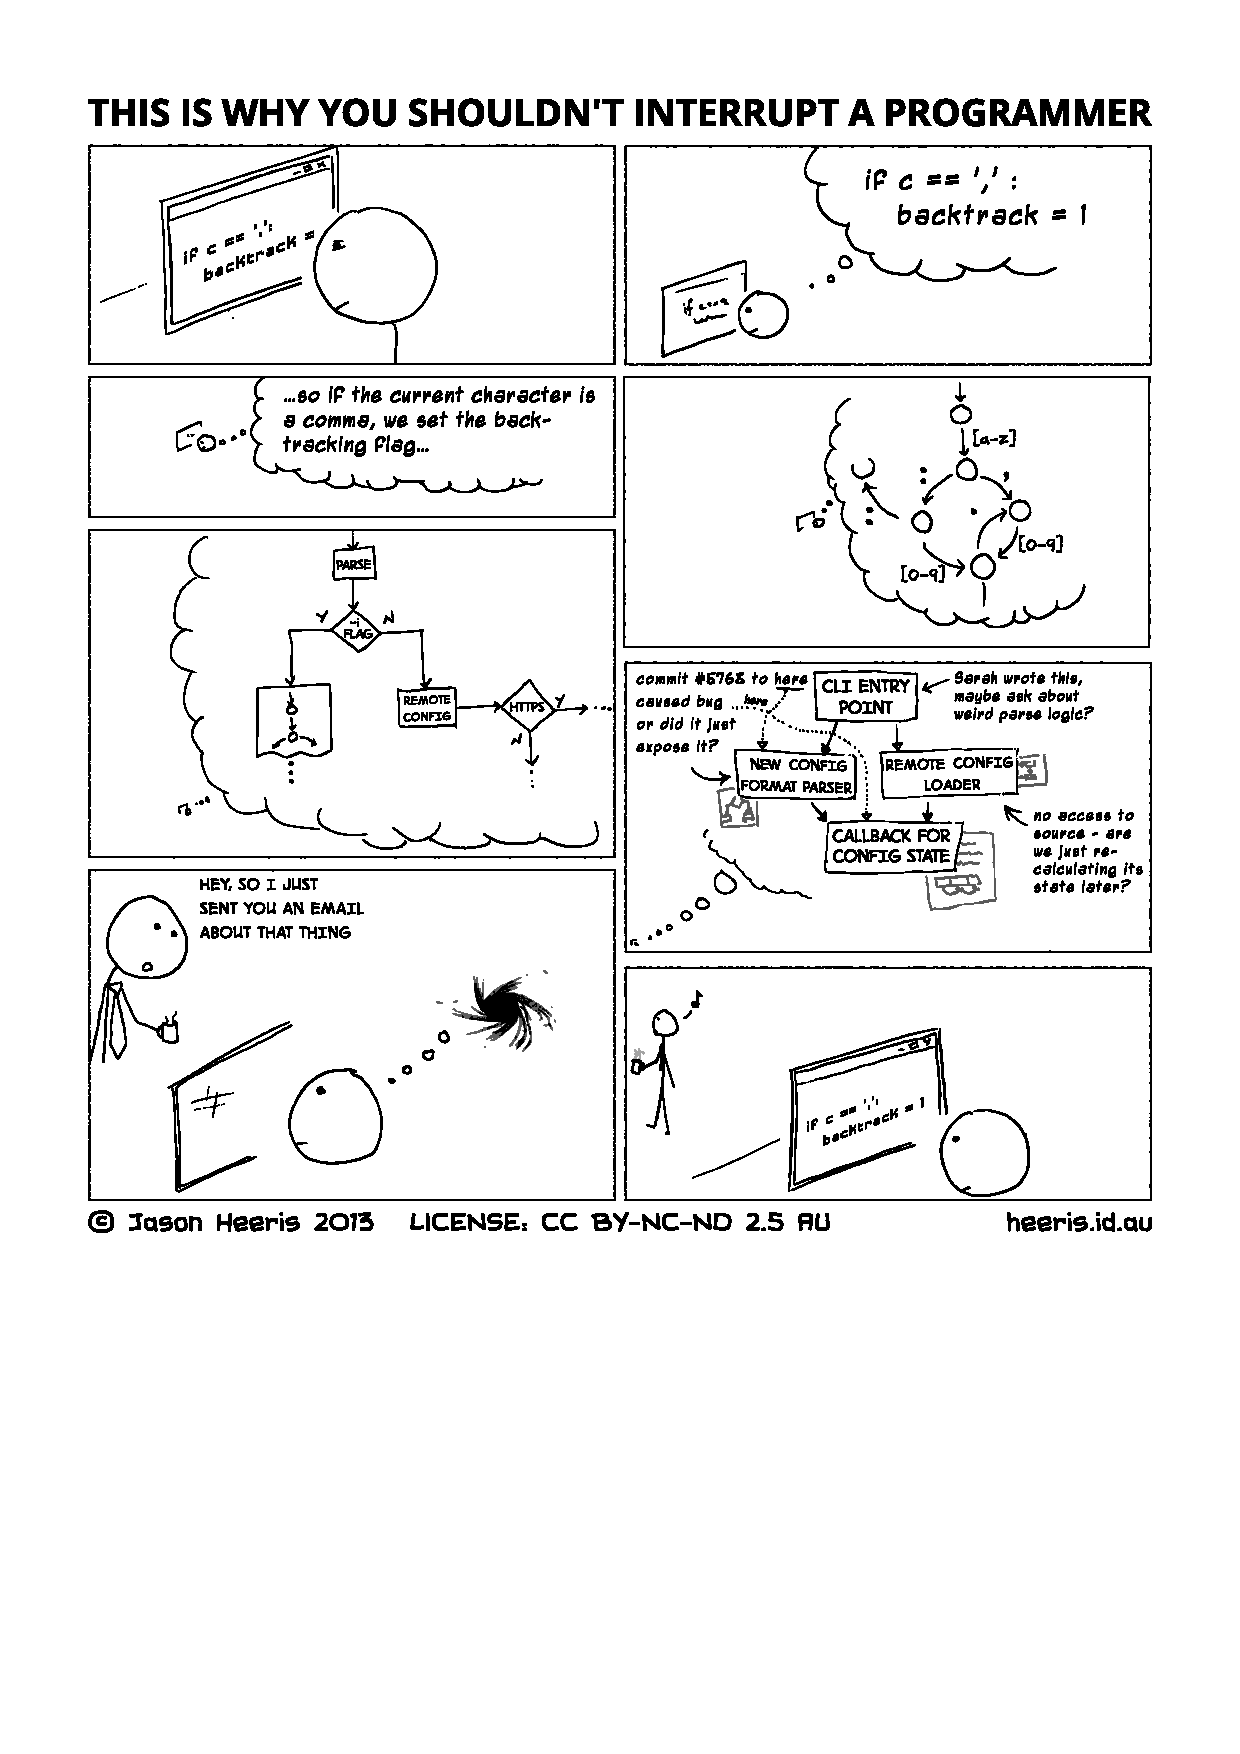
\includepdf[pages={1}, scale=.4, pagecommand={}]{data/ProgrammerInterrupted.pdf}
\begin{figure}[htp] \centering{
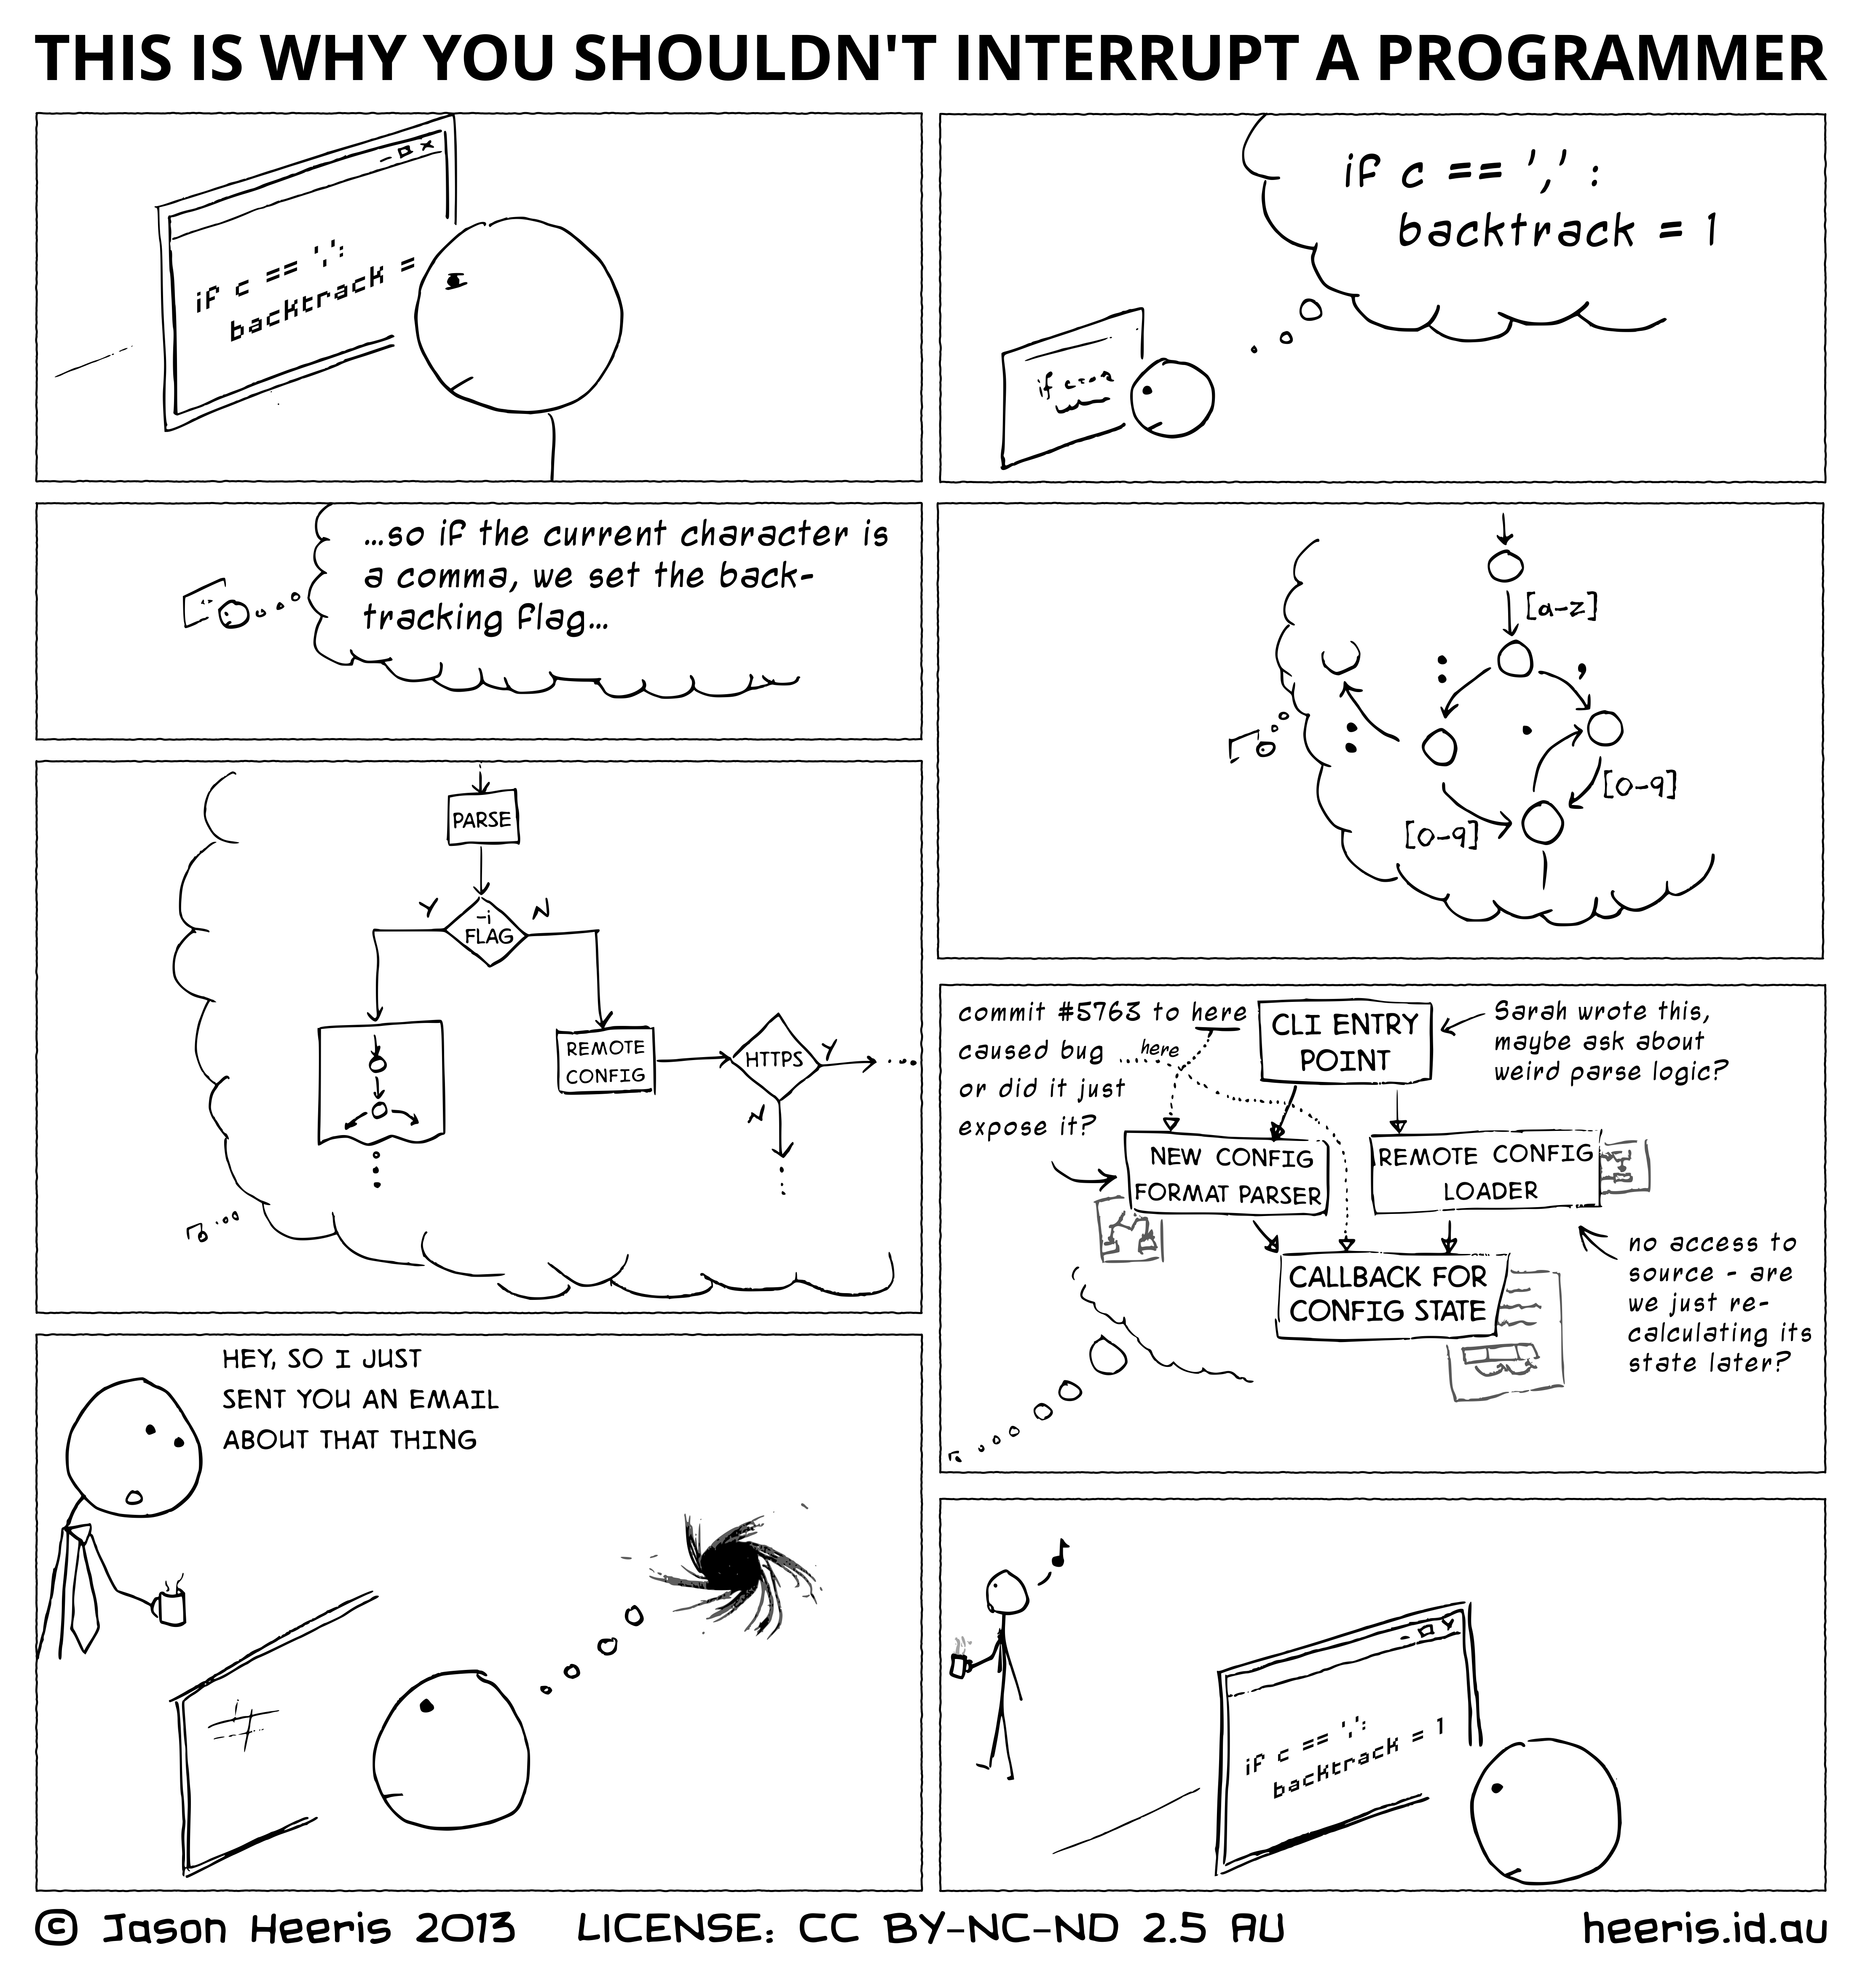
\includegraphics[scale=0.117]{data/ProgrammerInterrupted.png}}
\cite{programmerInterrupted}
\end{figure}  



\end{document}